\chapter{Evaluation} \label{chap:eval}

The previous chapter detailed the implementation of our design proposed in Chapter \ref{chap:design}, including the implementation of our \textit{Proactive} flow scheduler. This chapter describes the benchmarking tests that were carried out to evaluate our \textit{Proactive} flow scheduler against ECMP and Global First-Fit flow scheduling algorithms. Section \ref{sec:ExperiSetup} describes our experimental setup. Subsequently, in Section \ref{sec:BenchTraces}, we describe the nature of Hadoop job traces used for evaluation. Section \ref{sec:EvalOverview} gives a brief overview of the methodology followed in obtaining experimental results. Sections \ref{sec:EvalBandwidth} and \ref{sec:EvalJobCompletion} provide a comprehensive description regarding the evaluation of total average bisection bandwidth achieved by the different flow scheduling mechanisms and their effect on Hadoop job completion times. Finally, in Section \ref{sec:CriticalAnalysisEval}, we summarize our findings and critically analyse the same. 


\section{Experimental Setup} \label{sec:ExperiSetup}

The tests described in this chapter were all run on a Dell Server with 8 x 3.40GHz cores of Intel Core i7-4770 processor, 16 GB of RAM, and 475.4 GB of hard disk space running Ubuntu 14.04 LTS operating system. The Python implementation of our experiment used Python version 2.7. The Hadoop traces used in our evaluation were obtained by Neves \textit{et al.} \cite{neves2015mremu} on a real cluster of 16 identical servers, each having 12 x86 64
cores, a single HDD and 128 GB of RAM, interconnected via 1 Gbps Ethernet links, running Hadoop 1.1.2 on top of Red Hat Enterprise Linux 6.2 operating system. 

For running our network emulations, we used the \textit{Mininet} network emulator from its cs244 branch version, since it is compatible with \textit{Ripl-POX} controller that is used for ECMP routing, as discussed in \ref{sec:ControlImpl}. For the Hadoop emulation, we used the MRemu emulator \cite{MRemuRepo2015}, and used POX \textit{dart} \cite{POXdart} SDN controller for flow scheduling of the emulated Hadoop traffic.

\section{Benchmark Traces} \label{sec:BenchTraces}

The Hadoop job traces used to generate traffic in our experiment were obtained from the MRemu github repository \cite{MRemuRepo2015}. The same traces were used by Neves \textit{et al.} \cite{neves2015mremu} to evaluate the performance of MRemu. The traces have been obtained from the following applications which are a subset of the HiBench benchmark suite \cite{huang2011hibench}
\begin{itemize}
	\item Sort - This application sorts text input data which is generated via a RandomTextWriter. Sort is used frequently to benchmark Hadoop performance. 32 GB of data was sorted to obtain Job traces.
	\item PageRank - It implements the page-rank \cite{huang2011hibench} algorithm which calculates web page ranks by taking the number of reference links in the web page as a metric. Hence, PageRank serves as a large-scale indexing application. Neves \textit{et al.} configured PageRank to process 500K pages, totalling approximately 1 GB of input size; and used the Pegasus Project \cite{kang2009pegasus} implementation of PageRank to obtain job traces.  
	\item Nutch - It is part of Apache Nutch \cite{NutchWeb}, which is a scalable and flexible web crawler that uses the MapReduce model for indexing pages in  large-scale web search engines. Nutch was configured to index 5M pages, which totalled to approximately 8GB of input data.
	\item Bayesian Classification - Another canonical use of MapReduce is large scale machine learning. This application uses a classification algorithm for data mining and knowledge discovery called Naive Bayesian \cite{huang2011hibench}. It forms a part of Apache Mahout, which is a popular machine learning library. To obtain Hadoop job traces, 100K pages were configured to be processed by Bayesian Classification.
\end{itemize}

However, the Hadoop job traces in the MRemu github repository \cite{MRemuRepo2015} have not been classified according to the Hadoop applications that were run in the real cluster setup to obtain them. Therefore, in our evaluation of the effect of different flow scheduling mechanisms on total bisection bandwidth achieved and the respective Hadoop job completion times for different Hadoop job traces, we were not able to classify the different Hadoop traces on the basis of the HiBench applications that were used in order to obtain them. This is a limitation in our evaluation of the different routing mechanisms since different traces have achieved different levels of the network bisection bandwidth and we were not able to explore the causes for the same.    

\section{Evaluation Overview} \label{sec:EvalOverview}
We evaluated the effect of different routing mechanisms on the total bisection bandwidth achieved and Hadoop job completion times by running tests in the following manner

\begin{itemize}
	\item Firstly, we launched the POX controller with ECMP routing.
	\item While the ECMP controller was running, we launched the Mininet network emulation of a 16 host fat-tree topology with each host running the Hadoop emulation. 
	\item Subsequently, we stored the total bandwidth achieved and the total job completion times to disk, once the Hadoop emulation was over.
	\item We followed the same procedure listed above while running Global First Fit flow scheduling and our \textit{Proactive} flow scheduling in the POX controller instead of ECMP scheduling, and logged the total bandwidth achieved by the hosts in the emulation and their respective job completion times to disk.    
\end{itemize}

The above procedure was repeated for different Hadoop job traces and the results obtained are discussed in the following sections. 

\section{Evaluation of Total Bisection Bandwidth Achieved} \label{sec:EvalBandwidth}

After running benchmark tests as described in the previous section, we plotted the total throughput achieved for ECMP, GFF and \textit{Proactive} flow scheduling for different Hadoop job traces on the graph illustrated in Figure \ref{fig:RoutingVThroughput}. Global First-Fit flow scheduling was observed to outperform ECMP routing in all instances, achieving \textbf{24.21}\% more throughput on average than ECMP routing.  

 
\begin{figure}[!ht]
	\centerline{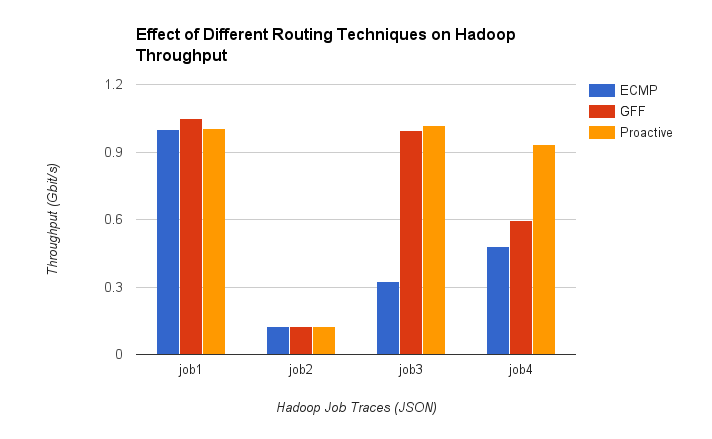
\includegraphics[scale=0.66]{graphics/chapter6/RoutingVThroughput.png}}
	\caption{Total throughput achieved by hosts running Hadoop job emulation in an emulated network with 1 Gbps links, grouped by the throughput achieved when running different Hadoop jobs for ECMP routing, Global First-Fit flow scheduling and \textit{Proactive} flow scheduling. On average, \textit{Proactive} flow scheduling was found to achieve \textbf{59.9}\% more bandwidth than ECMP routing and \textbf{11.6}\% more bandwidth than GFF flow scheduling.}
	\label{fig:RoutingVThroughput}
\end{figure}

Al-Fares \textit{et al.} \cite{al2010hedera} found Global First-Fit to outperform ECMP by achieving \textit{39}\% more of the total bisection bandwidth available in the network. The difference of \textit{15}\%, between our results and the ones obtained by Al-Fares \textit{et al.} might be attributed to the fact that we run our experiment on a single server, causing the GFF flow scheduler to perform slower due to limited computational resources. 

Our \textit{Proactive} flow scheduling mechanism was observed to perform significantly better than ECMP, achieving \textbf{59.9}\% more of the total bisection bandwidth available in the network than ECMP routing. In comparison to Global First-Fit routing, the \textit{Proactive} flow scheduler was comparable for the first two of the Hadoop Job traces, \textit{i. e.} \textbf{job1} and \textbf{job2} respectively, while for \textbf{job3} and \textbf{job4}, \textit{Proactive} flow scheduling outperformed Global First-Fit scheduling, as illustrated in Figure \ref{fig:RoutingVThroughput}. On an average, the \textit{Proactive} flow scheduler achieved \textbf{11.6}\% more of the total bisection bandwidth available in the network than Global First-Fit flow scheduling. 

Since we are not aware of the exact nature of the Hadoop job traces used in the evaluation of the \textit{Proactive} controller against ECMP routing and GFF flow scheduling, as described in \ref{sec:BenchTraces}, therefore, we cannot point out the reasons for \textit{Proactive} flow scheduling to outperform \textit{Global First-Fit} scheduling for \textbf{job3} and \textbf{job4} Hadoop traces respectively, while performing comparably to \textit{Global First-Fit} routing for \textbf{job1} and \textbf{job2} Hadoop traces, as illustrated in Figure \ref{fig:RoutingVThroughput}. Nonetheless, the results obtained substantiate our claim that \textit{Proactive} flow scheduling improves network performance by reducing the amount of control overhead in the network.      

The throughput readings used in Figure \ref{fig:RoutingVThroughput} were taken by re-running the tests described in \ref{sec:EvalOverview}, and taking the \textit{mode} of the throughput values obtained, so as to avoid \textit{Random Errors} in the values since the experiment was compute intensive. 

\section{Evaluation of Hadoop Job Completion Times} \label{sec:EvalJobCompletion}

As described in \ref{sec:EvalOverview}, we observed the Hadoop job completion times when traffic was routed following ECMP, Global First-Fit and \textit{Proactive} scheduling mechanisms respectively, for different Hadoop Job traces and plotted the readings on the graph illustrated in Figure \ref{fig:RoutingVJobCompletion}. We found the Hadoop job completion times to \textit{correlate} with the average bisection bandwidth achieved by hosts in the emulated network, when traffic was routed following the three flow scheduling algorithms, as described in the previous section.

\begin{figure}[!ht]
	\centerline{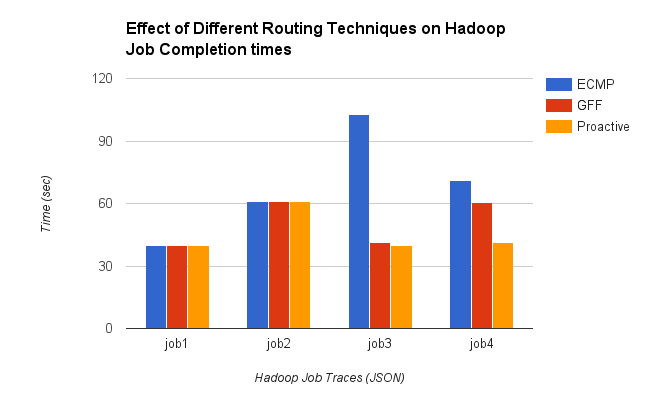
\includegraphics[scale=0.66]{graphics/chapter6/RoutingVJobCompletion.png}}
	\caption{Time taken to complete Hadoop job emulation by hosts in an emulated network with 1 Gbps links, grouped by Hadoop job completion times when running different Hadoop jobs for ECMP routing, Global First-Fit flow scheduling and \textit{Proactive} flow scheduling. \textit{Proactive} Flow scheduler achieves  lower Hadoop job completion times by \textbf{35.58}\% in comparison to ECMP routing and \textbf{10.07}\% in comparison to Global First-Fit flow scheduling.}
	\label{fig:RoutingVJobCompletion}
\end{figure}


\textit{Hadoop job completion times} were found to have an  \textbf{inverse correlation} with the \textit{total bisection bandwidth} achieved, indicating that flow scheduling mechanisms that achieve a higher bisection bandwidth result in lowering of Hadoop job completion times. We calculated Pearson product-moment correlation coefficient for average throughput achieved by different routing mechanisms as the dependent variable and the average time taken for Hadoop job completion by different routing mechanisms as the independent variable, and found the \textit{correlation coefficient} to be \textbf{-0.9981}, which is indicative of total negative correlation between the two. 

Moreover, Global First-Fit scheduling was found to lower Hadoop job completion times by \textbf{15.07}\% in comparison to ECMP scheduling, while the \textit{Proactive} Flow scheduler was found to lower Hadoop job completion times by \textbf{35.58}\% in comparison to ECMP scheduling and \textbf{10.07}\% in comparison to Global First-Fit flow scheduling. 

\section{Critical Analysis of Experiment Results} \label{sec:CriticalAnalysisEval}
As mentioned in Section \ref{sec:BenchTraces}, the Hadoop job traces used were a subset of the HiBench benchmark suite of MapReduce applications, specifically, Sort, Nutch, PageRank and Bayesian Classification, produced by Neves \textit{et al.} \cite{neves2015mremu}, made available on the MRemu github repository \cite{MRemuRepo2015}. However, they were not classified into their application types, hence we were not able to account for the reasons behind the difference in bisection bandwidth achieved by different Hadoop job traces as illustrated in Figure \ref{fig:RoutingVThroughput}; which is a limitation of our evaluation.  
\begin{figure}[!ht]
	\centerline{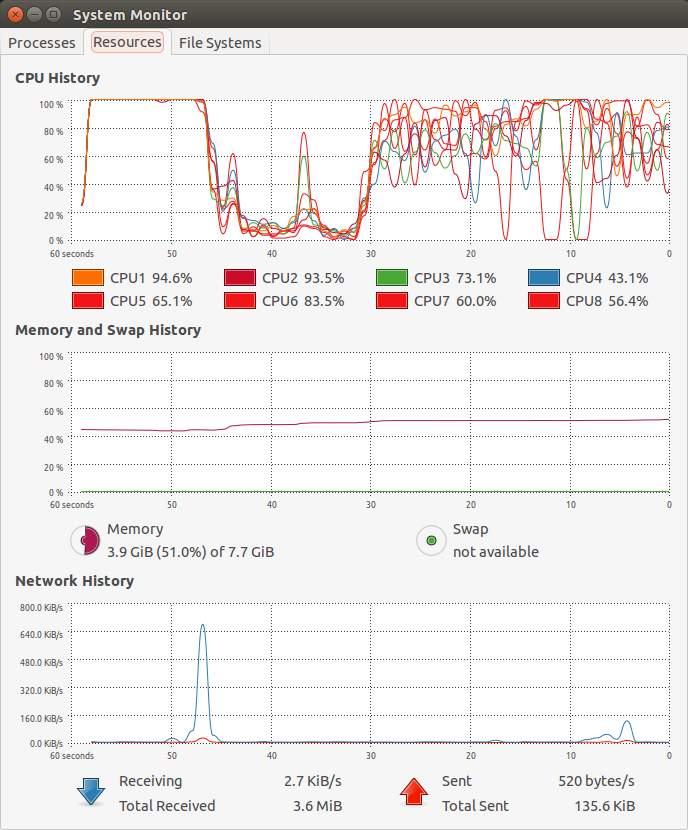
\includegraphics[scale=0.35]{graphics/chapter6/CPUUtilization.png}}
	\caption{A screenshot of the CPU utilization while the experiment was running on the server.}
	\label{fig:CPUutilization}
\end{figure}

Nonetheless, we were able to evaluate the bandwidth achieved and Hadoop job completion times for ECMP, GFF and our \textit{Proactive} flow scheduling mechanisms. Global First-Fit was found to achieve 24\% more aggregate bandwidth than ECMP. Al-Fares \textit{et al.} reported this difference to be 39\%. We speculate the difference in our findings to be attributed to the fact that our experimental setup involved a single server emulating 16 hosts arranged in a fat-tree topology, resulting in a  computation bottleneck as illustrated in Figure \ref{fig:CPUutilization}, which is a screenshot of the Ubuntu System Monitor utility, taken while the emulation was running, showing that at certain point of time, all 8 cores of our server used for the experiment were running at full processing utilization. 

We evaluated our \textit{Proactive} flow scheduling mechanism against ECMP and Global First-Fit flow scheduling, and observed an average gain of \textbf{59.9}\% and \textbf{11.6}\% in total bisection bandwidth achieved against ECMP and Global First-Fit flow scheduling respectively. Moreover, \textit{Proactive} flow scheduling achieved faster Hadoop job processing times by \textbf{35.58}\% and \textbf{10.07}\% in comparison to ECMP and Global First-Fit flow scheduling, highlighting the potential of \textit{Proactive} Network configuration approaches to optimize performance of Big Data applications. Moreover, we found the total bisection bandwidth and Hadoop job completion times to be negatively correlated by Pearson's correlation coefficient of \textbf{-0.99}, which underlines the huge potential of \textit{Reactive} and \textit{Proactive} Network configuration to enhance the performance of Big Data processing applications in a data centre network.